\chapter{Methodology}
\label{chap:meth}

This chapter starts with the analysis of requirements for the implemented
software. In the second section of the chapter I will discuss possible
approaches to adapt an external state machine to Phantom OS persistency model.
The last section describes the implementation and design decisions in detail.

\section {Requirements analysis}

As previous chapters of this paper suggest, the goal of this paper is to create
an implementation of a TCP suitable for a persistent system. More precisely, I
target a port of Phantom OS to Genode OS framework. This section contains a
list of requirements that I will follow while designing my own protocol
implementation.

\subsection {Transparency for client applications}
Persistent support systems (PSSs) aim to make development of applications
easier. The PSSs provide their clients with an abstraction of an uninterrupted
execuiton. In a real world, however, a computer system may experience
downtimes. The point of a PSS is to hide these downtimes from applications that
use it. Such hiding of undesired effects is generally called
\textit{transparency}.

As discussed in Section \ref{sec:int:phantom}, the current implementation of
networking stack is not transparent for the applications residing in PVM.
Application designers should foresee existence of these errors and write
handlers for them. To make PoG port really orthogonally persistent these errors
should be hadled at PSS level, not by clients.

That means that the state of TCP connections should be the same before a
shutdown and after a reboot. To achieve that a persistent TCP implementation
should either (1) backup and restore connections state or (2) make the
disappearance of a remote peer invisible for application on the other end of
the connection. Of course, restoration of the state should be done before
returning control to applications.

(1) can be achieved with reestablishing connections on startup. However, the
remote peer should be ready to the reestablishment request. This is problematic
in case when a persistent host plays role of a server in a client-server
communication. (2) can be achieved with use of an message broker that will
mimic an alive host with full TCP input queue. Thus it will keep the connection
alive but prohibit sending packets to the channel. Another way to achieve (2)
is to send a control message to the remote socket. The remote TCP in this case
should efficiently do the same thing as a message broker did. It should mimic
live connection that cannot accept data. The drawback of this approach is that
to exchange control messages both communicating peer should have enhanced TCP
stack.

\subsection {Robustness to rollbacks}

Phantom OS uses full-memory snapshots of PVM memory space to provide
persistence for its clients. Snapshots are taken in a live mode so that
processes inside the VM continue to run. Due to the two previous facts,
computational operations of PVM applications can be executed more than once.
For example, assume that an application receives packets A, B, and C.  Assume
that after packet A is received, snapshot is performed. While it was on
progress, the application receives packet B. After the snapshot was made,
applications reveives packet C and immediately after this machine goes down.
After the snapshot would be restored the application will have no knowledge
that it already received packets B and C. Thus the application will send ACK
packet for A, which will result in error because the remote peer does not
expect this ACK. Moreover, it is unable to retransmit this packet, since it is
not exist in remote TCP's retransmission queue, because it was already
acknowledged when the application received B and C.

Phantom OS snapshot mechanism takes into account that snapshot is not a atomic
process. Thus, in usual case it would handle reception of packet B properly,
i.e. the client application would know that B was received. But in case of 
PoG the TCP stack is not stateless like Phantom kernel but still transient.
Therefore, if TCP receives a packet but does not passes it to the application
before restart, this packet may be lost. The remote peer expects that the
application processed it but the application never received it because TCP did
not finish delivering it to the application.

Three solutions exist that may solve the problem above. The first is to refrain
from sending acknowledgment packets if a received packet is not included in any
snapshot. However, this will either dramatically increase the number of
retransmissions in a network, which will result in reduced network performance
or it will require doing snapshots very often. In such case a snapshot should
be performed each 50ms to avoid extra network congestion at all. However, in
PoG a snapshot runs for around 10 seconds. This approach is not acceptable with
such a long snapshot.  

The second solution is to keep in persistent memory a buffer that will store
all packets that TCP clients had not consumed yet. In this case persistent
memory can be a regular file or snapshotted memory space. 

The third approach is to have a message broker inside a network that will
function similarly to the buffer in the second approach. The broker can save
all acknowledged packets in a network, and flush its queue when it detects that
receiving host has done a snapshot. ICMP messages or some similar stateless
network protocol could be useful to notify the broker about the end of the
snapshot process.

\subsection {Usefullness}

Phantom OS is already capable of restoring sockets in CLOSED and LISTEN states.
For a Genode implementation of a persistent TCP to be useful it should work for
the same or bigger set of states. Even if the developed software will only
support the same set of states the fact that the software is implemented as a
Genode component will greatly improve maintainablility of the software.

\subsection {Compatibility with existing protocols}

The last design goal is not directly related to providing persistent I/O
abstraction to the clients of a network stack. Since snapshotting is a very
popular technique for implementing persistent systems, and Genode is actively
used to develop various operating systems, it is probable that some other
developers might want to use persistent TCP in their software.

That means that result of this work should be a standalone application that
works without Phantom and is flexible enough to support all use cases that may
arise. Fortunately, Genode's component-based architecture helps greatly with
it. Another reason to make persistent TCP implementation a standalone
application is that the PoG port is not yet ready for me to experiment with it.

Another thing that should be addressed in the design of the API of the system,
is easy migration from non-persistent TCP stacks that are already available in
Genode, namely lwip and lxip. To do this I intend to design API very similar to
regular sockets or even exactly the same, but with different call semantics. I
also plan to add a Virtual File System (VFS) plugin that will expose sockets as
regular files because this is the way how Genode developers suggest
integrating sockets into the Genode ecosystem since version 18.11. With such
implementation, even relinking of existing binary will be not needed. The only
thing user would need is to change the configuration of the init Genode
component.

\section{On persisting of finite state machines}
\label{sec:meth:fsms}

Most TCP implementations implement logical state of the sockets as finite state
machines. Since the goal of the paper is to create a persistent TCP
implementation, it might be useful to consider how an arbitrary FSM can be
snapshotted to restore it later to the same state from the snapshot. 

The most straightforward and universal way to achive the desired outcome is to
use a full-memory snapshot of a running process. Full-memory snapshot should
include stack and address space. Also it should include current context, i.e.
general-purpose registers and the program counter. Obtained snapshot should be
stored in a persistent memory and loaded to the apropriate memory on restore.
In principle, this approach would work for any running process. A drawback of
this approach is that an operating system should provide mechanisms to allow
such manipulations with address spaces.

The second approach is to directly access current state of the FSM. Usually FSM
are implemented on C and C++ as structs or classes holding current state as an
value of an enumerable type. If it is possible to access these structures
directly, simple saving and loading them would work. In some cases, for example
sockets, there are several state machines: one per socket. In such cases FSMs
should be registered at the supervisor that controls inputs and stores FSM
structures.

The last approach requires knowing of internal functioning of an FSM. When the
set of all possible states and transitions of FSM is known in advance, it is
possible to implement FSM with the same transitions. When the tracking FSM is
provided with the same inputs as the target one states of both FSMs should be
in sync. Assessing state of the tracking FSM will allow observer to determine
state of the target FSM.  Moreover, tracking of inputs greatly helps in
restoration phase. To restore state of the target FSM it is enough to provide
it with the same inputs once again. This approach is useful when an FSM does
not have a centralized state or when it cannot be easily accessed.

\section{Implementation process}

\subsection{Components of Genode network stack}

\begin{figure}
    \centering
    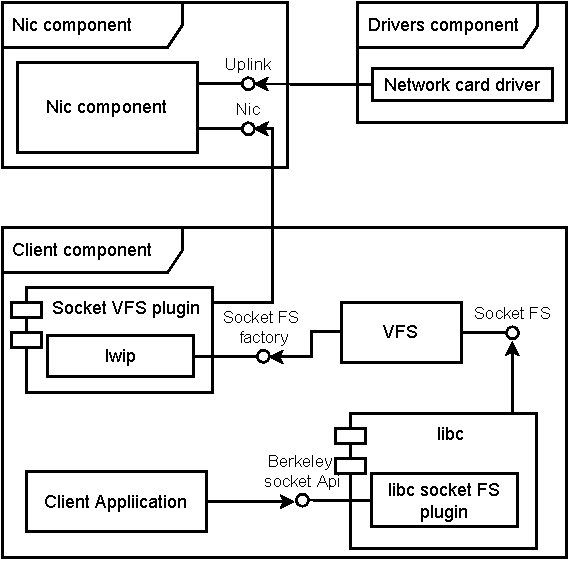
\includegraphics[]{figs/genode-network-stack.pdf}
    \caption{Components of Genode network stack}
    \label{fig:net-components}
\end{figure}

Before discussing the implementation details of developed persistent TCP stack
it is necessary to consider how Genode network stack works. Figure
\ref{fig:net-components} depicts components and libraries that are required to
enable a network access for a client application. In this diagram Nic stands
for Network interface controller. Nic component is a mediator for packets that
are produced and consumed by applications and network drivers. As can be seen
from the diagram, Nic interface provides two RCP interfaces: the Uplink
interface is used by network drivers, and the Nic interface is used by client
applications. Nic interface exposes network packets as Ethernet frames.

The Nic RPC interface is almost never used directly. Instead most applications
tend to use Berkeley sockets API, which include well-known functions socket(),
bind(), connect(), listen, and others. This API is provided by libc. Genode's
libc is based by FreeBSD libc and its functions are implemented by so-called
libc plugins. Berkeley sockets API is implemented in the socket\_fs plugin.
This plugin depends on Genode VFS. The plugin expects VFS to expose each socket
as a set of virtual files.

The socket\_fs plugin should be used in conjunction with a socket VFS plugin. 
Such VFS plugin generally is merely an adapter between a Nic session and port
of some popular TCP stack. A port is denoted by "lwip" on the Figure
\ref{fig:net-components}. For now, two TCP ports available in Genode -- lxip,
which is a port of Linux TCP/IP stack, and lwip. Usually TCP stack is
statically linked with a VFS plugin, and VFS plugins are shared libraries which
are loaded in runtime.

Each Genode component has an initial configuration that is written as an XML
"config" node. The node also may contain configuration for VFS, if a component
needs one. Configurations for VFS and libc are located at "vfs" and "libc"
sub-nodes of "config". Each VFS directory can have a plugin that will handle
access to the directory and all its subdirectories and files. Plugins libraries
are resolved in the runtime when a component initializes. To use libc with a
socket VFS plugin component should place a VFS plugin to some directory and
pass path to this directory to the libc config. A minimal example configuration
for Genode component that is able to use network is given in the Appendix
\ref{appex:conf-sample}

I had a hypothesis that persistent TCP stack can be implemented as a VFS plugin
wrapping another VFS plugin. The inner VFS plugin would provide a "real" 
TCP interface, and the outer plugin would supervise the inner one to save and
restore its state as needed. I decided to name the plugin PTCP from "persistent
TCP". PTCP uses lwip VFS plugin. PTCP is dynamically linked with the plugin, at
the runtime it loads vfs\_lwip shared library. This dynamic linkage was done by
design, with the assumption that system that has components using PTCP can also
have components that use plain lwip VFS plugin, since it is popular among
Genode software.

\subsection{Snapshot structure}

The PoG port was not ready during the most of the time this work was in
progress. However, the technique this port uses to achieve persistence was
known in advance. The technique is snapshotting just like in plain Phantom OS.
To use snapshotting I needed to decide what data should be included in a
snapshot. I tried several different approaches with respect to the snapshot
content. The content of a snapshot is discussed in detail in this subsection.

The first attempt to snapshot a TCP implementation concluded in saving the
state of socket state machine. This is the second approach proposed in Section
\ref{sec:meth:fsms}. For simplicity I decided to start with saving and
restoring a specific VFS plugin -- lwip. lwip represents a socket as a protocol
control block (PCB). PCB is a structure that holds values that are required for
protocol functioning. For example, TCP PCB encapsulates current state, SEQ
number, ACK number, and several other fields. lwip keeps all PCBs in the few
linked lists. References to these lists are located at static section of lwip
binary.

The challenge was to access the lists from the PTCP plugin. PTCP can access the
address space of the inner plugin but the problem was that lwip is statically
linked to the vfs\_lwip plugin. Moreover, all lwip symbols are erased during
the linkage from the binary. The only symbol exposed from vfs\_lwip is a
function that returns a factory for lwip plugin instances. To overcome this
issue I reconfigured vfs\_lwip to include lwip as a shared library. With this
reconfiguration I was able to access lwip internal structures from PTCP plugin.
Both vfs\_lwip and PTCP used the lwip shared library. The VFS pluigins existed
in the same Genode component, so they used the same "instance" of lwip.
Relationships between the libraries are presented at the Figure
\ref{fig:lib_deps}. There lwip\_dl.lib.so denotes lwip in form of shared
library.

\begin{figure}
    \centering
    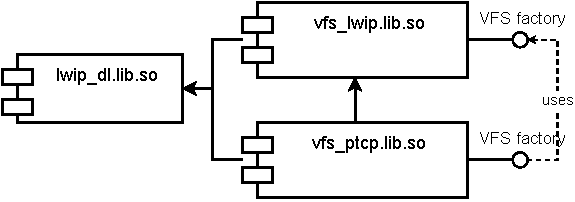
\includegraphics[]{figs/ptcp_libs.pdf}
    \caption{Relationships between the libraries comprising PTCP}
    \label{fig:lib_deps}
\end{figure}

After I manage to access the internal state of lwip in form of PCBs I started
implementing saving it to persistent storage. A PCB is a C structure and I
tried to save each PCB corresponding to socket field by field to a file.
However, in the process of implementing I discovered the two issues that made
me abandon this approach. The first problem that I discovered was a rather
complex structure of the PCBs. The tcp\_pcb structure includes more than 60
members and some of them are not atomic values but rather nested structures or
buffers. Also list of members of tcp\_pcb can vary depending on compile-time
config. The second issue was that despite my assumption sockets state was
stored not solely on lwip PCB lists but also at the lwip VFS plugin level and
even in libc. Therefore even if I would proceed with snapshotting lwip internal
structures I would not achieve desired effect.

To mitigate the two issues above I decided to abandon the idea of saving state
holding structures on the field-by-filed basis and instead proceed with saving
and loading memory that belongs to them.

\subsection{Approach with memory}
As a second approach I tried to save memory pages that belong to network stack
and restore them on component startup. Genode manages virtual memory with use
of Allocator class instances. I have subclassed the base Allocator class and
created a class that was able to track virtual addresses it allocated, save
allocated regions to a file, and load them back to virtual memory. I applied
this allocator so that it saved and restored heap dataspaces related to libc,
lwip VFS plugin and lwip itself.

At this point I faced a problem related to restoration of heap space. If a heap
space is prepopuilated before an allocator is passed to its user it will never
use this space. The allocator will never return adresses belonging to the
address range of the space in response to the user's allocation request. After
I understood the problem I changed the implementation so that it overwrote an
address range \textit{after} it was returned in response to user's request. That
is the program detected that the TCP stack finished its initialization and then
overwrote its address space with memory from previous boot of the system.
However, this approach did not work by the two reasons. 

The first reason was the presence of the kernel capabilities inside the address
space. Capabilities are used throughout almost each part of the Genode OS
framework. In fact, the component can not exist without using at least one
capability, and can not execute any code without using at least three - namely
Parent, CPU and RAM capabilities. lwip VFS plugin should use eight more
capabilities to use Nic RPC interface. Each allocated address range consumes
one dataspace capability to use virtual memory service RPC interface. This
ubiquity of capabilities and the fact that they become invalid after restart
make straightforward saving and loading of component's memory to disk
impossible. This approach becomes even more complicated if a snapshotted
component uses shared memory. For example, Nic servers use zero-copy packet
delivery mechanism to increase memory throughput. This mechanism implies
establishment of shared memory between client and server components.

The second and the main issue with the raw memory saving approach is that
layout of structures in the memory is undefined. The layout depends on order
of allocation requests and presence of Address space layout randomization
(ASLR). The interface of Allocator class does not allow the allocator determine
the purpose of allocation, i.e. what structure will be placed in the newly
created dataspase. These two issues explain why I decided to stop work in this
direction and decided to shift focus to a completely different approach.

For example, a dataspace might be shared with other components that
are not persisted. In this case persistent component expects its sibling to
write something to the dataspace they used for memory-mapped communication
earlier, and the sibling is unaware of any communications before power loss.

\subsection{Observer state machine}

The main idea of the new approach was to build a tracker that will know the
internal state of every socket without directly accessing those states. This
idea is the third approach that was proposed in section \ref{sec:meth:fsms}. 
We can treat each socket as a graybox where the inputs are user-called
functions and TCP packets from network. The outputs of this box are packets
that are scheduled for sending at the Nic server and data chunks delivered to
clients of TCP stack.

The libc transforms user calls to Berkeley socket API into file access
operations. This operations are processed by Genode VFS. It delegates
operations to its plugins. In our case all socket operations are processed by
the PTCP plugin. To enable PTCP track VFS calls I created a wrapper around
FS factory exposed by the PTCP inner plugin. This wrapper creates a new
proxy filesystem that delegates processing all calls to FS returned by the
inner plugin. The proxy FS is equipped with a tracking delegate that notifies
the tracker about each accessed file. The tracker keeps a one metadata
structure per each socket. When a tracking delegate notifies the tracker it
searches the socket metadata that corresponds to the accesses file. Then the
tracker updates the structure according to the new socket state.

To enable tracking and control for the arriving network packets I added a
secondary Nic server that scans headers of incoming packets and notifies the
tracker. The tracker is the same one that was discussed above. The presence of
tracker allows PTCP to intercept incoming packets without changing code of the
inner plugin. 

To restore state of the sockets I added a client library that is used on
component startup. During initialization the library reads a snapshot, reopens
each socket present in the snapshot, and brings them to the last known state.
Restoration of the state is performed with the sequence of calls to Berkeley
socket API, and RPC calls to the proxy Nic server. The proxy Nic is responsible
for restoration of those parts of socket state that can not be set by user. For
example, these parts include sequence and acknowledgements numbers. To restore
those values the Nic proxy acts similar to the NAT mechanism in routers. But 
instead of changing source and destination ports values in TCP packet headers
the Nic proxy changes headers so that the remote side of the connection would
recognise the newly opened socket as the old one. The idea of proxy was highly
inspired by the use of Linux kernel packet filters in \cite{rocks_racks}.

% TODO Illustration fot architecture of the system

\subsection{Snapshot location}

The goal of this paper is to design a persistent networking stack suitable for
Phantom OS. Due to this, it is possible to include a snapshot of the TCP stack
into the Phantom VM snapshot structure. However, I decided that a persistent
network stack can be useful not only for the Phantom OS but also for other
persistent systems. These systems can use other mechanisms for persistence. Due
to this, I decided to make an abstract interface that has functions for saving
and loading binary data from persistent memory.

For simplicity, the only implementation of this service saves its state
directly to the hard drive volume attached to VM. An implementation that saves
and loads data using the Phantom snapshotting mechanism is currently in
progress.

